\documentclass[11pt, oneside]{article}   	% use "amsart" instead of "article" for
\usepackage{geometry}            	% See geometry.pdf to learn the layout options. 
\geometry{letterpaper, margin=1in}              	% ... or a4paper or a5paper or ... 
\usepackage{graphicx}				% Use pdf, png, jpg, or eps§ with pdflatex; use 	
\usepackage{amssymb}
\usepackage{booktabs}
\usepackage[font=small,labelfont=bf]{caption}
\usepackage{titling}
\usepackage[printwatermark]{xwatermark}
\usepackage{xcolor}
\usepackage{graphicx}
\usepackage{tikz}
\usepackage{lipsum}
\usepackage{multirow}

\setlength{\droptitle}{-8em}

\usepackage{fancyhdr}
\pagestyle{fancy} % enable fancy page style
\fancyfoot[R]{ % right
%    \includegraphics[scale=0.9]{../ARSlogo.png}
}

\newenvironment{noindlist}
 {\begin{list}{\labelitemi}{\leftmargin=1em \itemindent=0em}}
 {\end{list}}

% \rhead{ \begin{flushleft} \vspace{-1cm} {\color{red} DRAFT }  \vspace{-1cm} \end{flushleft} \includegraphics[width=1cm]{/home/markrobertson/mrworkspace/reports/Tuolumne/figs/logo.png}}

\rhead{ \begin{flushleft} \vspace{-1cm} {\color{red} DRAFT }  \vspace{-1cm} \end{flushleft}}


\title{ {\color{red} DRAFT } \\ \textbf{\VAR{REPORT_TITLE|e}} \\
Water Year \VAR{WATERYEAR|e} \\ \VAR{START_DATE|e} to \VAR{END_DATE|e} \VAR{FORE_DATE|e}
}


\author{USDA Agricultural Research Service, Boise, Idaho \\
NASA Jet Propulsion Lab, Pasadena, California \\
\emph{in cooperation with} NRCS National Water and Climate Center, Portland, Oregon\\
\emph{and} U.S. Bureau of Reclamation, Sacramento, California} 
\date{}						


\begin{document}
\maketitle

% \begin{tikzpicture}[remember picture,overlay]
% \node[anchor=west,inner sep=0pt] at (-1.5,4cm) {\includegraphics[height=3.5cm]{/home/markrobertson/mrworkspace/code/SNOWAV/report/figs/logo.png}};
% \end{tikzpicture}

\vspace{-1.2cm}
\section{Summary}
\VAR{SUMMARY|e}

\begin{table}[h!]
	\caption*{\textbf{Basin Snow Storage}}
	\centering
	\begin{tabular}{l c c c c c }
		\toprule
		
		\multirow{2}{*} {\bf{Basin} }	& SWE & SWE (avail) & SWE (mean) & $\Delta$SWE  \\ & [\VAR{UNITS|e}] & [\VAR{UNITS|e}] & [mm] & [\VAR{UNITS|e}]	\\
		
		\midrule
		Extended Tuolumne	& \VAR{TOTAL_SWE|e} & \VAR{TOTAL_SWE_AV|e} & \VAR{TOTAL_PM|e} & \VAR{TOTAL_SWEDEL|e} \\
		Tuolumne	    	& \VAR{SUB1_SWE|e}	& \VAR{SUB1_SWE_AV|e}  & \VAR{SUB1_PM|e} & \VAR{SUB1_SWEDEL|e} \\
		Cherry	   			& \VAR{SUB2_SWE|e}	& \VAR{SUB2_SWE_AV|e}  & \VAR{SUB2_PM|e} 	& \VAR{SUB2_SWEDEL|e}  \\
		Eleanor	        	& \VAR{SUB3_SWE|e}	& \VAR{SUB3_SWE_AV|e}  & \VAR{SUB3_PM|e} & \VAR{SUB3_SWEDEL|e} 	 \\
		\bottomrule
	\end{tabular}
	\label{tab:snotel}
\end{table}


\begin{table}[h!]
	\caption*{\textbf{Basin Surface Water Inputs}}
	\centering
	\begin{tabular}{l c c c c c }
		\toprule
		
		\multirow{2}{*} {\bf{Basin} }	& SWI & Melt & Rain & $\%$ Rain \\ & [\VAR{UNITS|e}] & [\VAR{UNITS|e}] & [\VAR{UNITS|e}] &  \\
		
		\midrule
		Extended Tuolumne	& \VAR{TOTAL_SWI|e} & \VAR{TOTAL_MEL|e}  & \VAR{TOTAL_RAI|e} & \VAR{TOTAL_RAT|e}  \\
		Tuolumne	    	& \VAR{SUB1_SWI|e}	& \VAR{SUB1_MEL|e}  &  \VAR{SUB1_RAI|e} & \VAR{SUB1_RAT|e} \\
		Cherry	   			& \VAR{SUB2_SWI|e}	& \VAR{SUB2_MEL|e}  & \VAR{SUB2_RAI|e} & \VAR{SUB2_RAT|e} \\
		Eleanor 	        & \VAR{SUB3_SWI|e}	& \VAR{SUB3_MEL|e}  & \VAR{SUB3_RAI|e} & \VAR{SUB3_RAT|e} \\
		\bottomrule
	\end{tabular}
	% \caption{yupperdep}
	\label{tab:snotel2}
\end{table}

\begin{itemize}
	\item[] SWE: Snow Water Equivalent, snow storage in the basin
	\item[] SWE (avail): amount of snow at 0$^{\circ}$C, which will melt with any additional energy inputs
	\item[] SWE (mean): basin-wide mean SWE, as a depth
	\item[] $\Delta$SWE: change in SWE during the reporting period
	\item[] SWI: Surface Water Inputs, the combination of snowmelt and rain
	\item[] Cold Content: energy required to bring the snowpack to 0$^{\circ}$C
\end{itemize}

\clearpage

%%  \section{Current Model Results (through \VAR{END_DATE|e}, 2017)}
\section{Results}
\VAR{RESULTS_SUMMARY|e}

% SWE change
\begin{figure}[htbp]
\begin{centering}
	% \hspace*{-.7in}
	\includegraphics[width=0.92\textwidth]{\VAR{FIG_PATH}\VAR{CHANGES_FIG}}
	\caption{Change in SWE during the reporting period.}
	\label{fig:RESULTS}
\end{centering}
\end{figure}

% SWI
\begin{figure}[htbp]
\begin{centering}
	% \hspace*{-.7in}
	\includegraphics[width=0.92\textwidth]{\VAR{FIG_PATH}\VAR{SWI_FIG}}
	\caption{Current Surface Water Inputs (SWI) for the reporting period. Hatching indicates the portion of SWI that came as snowmelt, rather than rain.}
	\label{fig:SWI}
\end{centering}
\end{figure}

% SWE distribution
\begin{figure}[htbp]
\begin{centering}
	% \hspace*{-.7in}
	\includegraphics[width=0.9\textwidth]{\VAR{FIG_PATH}\VAR{RESULTS_FIG}}
	\caption{Current distribution of SWE and cold content.}
	\label{fig:RESULTS}
\end{centering}
\end{figure}

% SWE elevation
\begin{figure}[htbp]
 \begin{centering}
 	% \hspace*{-.7in}
 	\includegraphics[width=0.9\textwidth]{\VAR{FIG_PATH}\VAR{ELEV_FIG}}
 	\caption{Current SWE per elevation band for each sub basin.}
 	\label{fig:RESULTS}
 \end{centering}
\end{figure}



\clearpage
% 
\begin{figure}[htbp]
	\begin{centering}
		% \hspace*{-.7in}
		\includegraphics[width=0.9\textwidth]{\VAR{FIG_PATH}\VAR{TOTALS_FIG}}
		\caption{Daily SWE and SWI basin totals.}
		\label{fig:TOTALS}
	\end{centering}
\end{figure}

\clearpage
\section{ASO Flight Update, \VAR{END_DATE|e}, 2018}

% SWE change
\begin{figure}[htbp]
	\begin{centering}
		% \hspace*{-.7in}
		\includegraphics[width=0.92\textwidth]{\VAR{FIG_PATH}\VAR{CHANGES_FLT_FIG}}
		\caption{Change in SWE as a result of the ASO flight.}
		\label{fig:RESULTS}
	\end{centering}
\end{figure}

\begin{table}[h!]
	\caption*{\textbf{Snowpack Storage Update}}
	\centering
	\begin{tabular}{l c c c c c }
		\toprule
		
		\multirow{2}{*} { }	& SWE  & SWE (mean)  \\ & [\VAR{UNITS|e}]  & [mm] 	\\
		
		\midrule
		Pre-flight			& \VAR{PRE_SWE|e} 		& \VAR{PRE_PM|e} 	\\
		Post-flight	    	& \VAR{TOTAL_SWE|e}  	& \VAR{TOTAL_PM|e} 	\\
		Difference 			& \VAR{FLT_SWEDEL|e}  	& \VAR{DIFF_PM|e} 	\\

		\bottomrule
	\end{tabular}
	\label{tab:snotel}
\end{table}



\vspace{2cm}

\noindent\textbf{STATEMENT OF INTENT:} This report is created as a product of a research agreement between the USDA-ARS Northwest Watershed Research Center and the NRCS National Water and Climate Center. 
This report is intended to demonstrate the capabilities of real time physically-based snow modeling and the tools being developed within the scope of that research agreement.
USDA-ARS provides the data to the best of its knowledge and shall not be liable for any consequences of any kind, including, but not limited to, lost revenues and profits, that arise from using the products provided.
\vspace{0.5cm} \\
\noindent
Contact: \\
\hspace{2cm} Mark Robertson, mark.robertson@ars.usda.gov, (208) 422-0729 \\
\hspace{2cm} Scott Havens, scott.havens@ars.usda.gov, (208) 422-0739 

\end{document}  